% arara: xelatex: {synctex: true}
% arara: indent: {overwrite: yes}
\documentclass[]{IMTexam}

\usepackage[enums]{IMTtikz}

\givecredits
\author{Isabella B.}
\USPN{11810773}
\date{}
\lecture{Física I} % disciplina
\lcode{4302111}
\hwtype{Resolução} % o que é
\examname{Lista 6} % prova

\begin{document}

\maketitle

\begin{questions}

	\question Em um parque de diversões um brinquedo conhecido como \textit{Spinning Terror} consiste de um grande cilindro vertical que gira tão rápido que todo mundo que está dentro fica grudado na parece quando o piso do cilindro é removido.

	\begin{enumerate}
		\item Desenhe o diagrama de forças sobre um indivíduo de massa $ M $ que está grudado à parede do cilindro de raio $ R $ girando com velocidade angular $ \omega $.
		\item Admitindo que o coeficiente de atrito é $ \mu $, determine qual o valor mínimo da velocidade angular $ \omega $ que permite que o brinquedo seja seguro.
		\item Estime quantas voltas por segundo corresponde a essa velocidade angular mínima.
	\end{enumerate}

	\begin{solution}

		\topenum
		\begin{multi}

			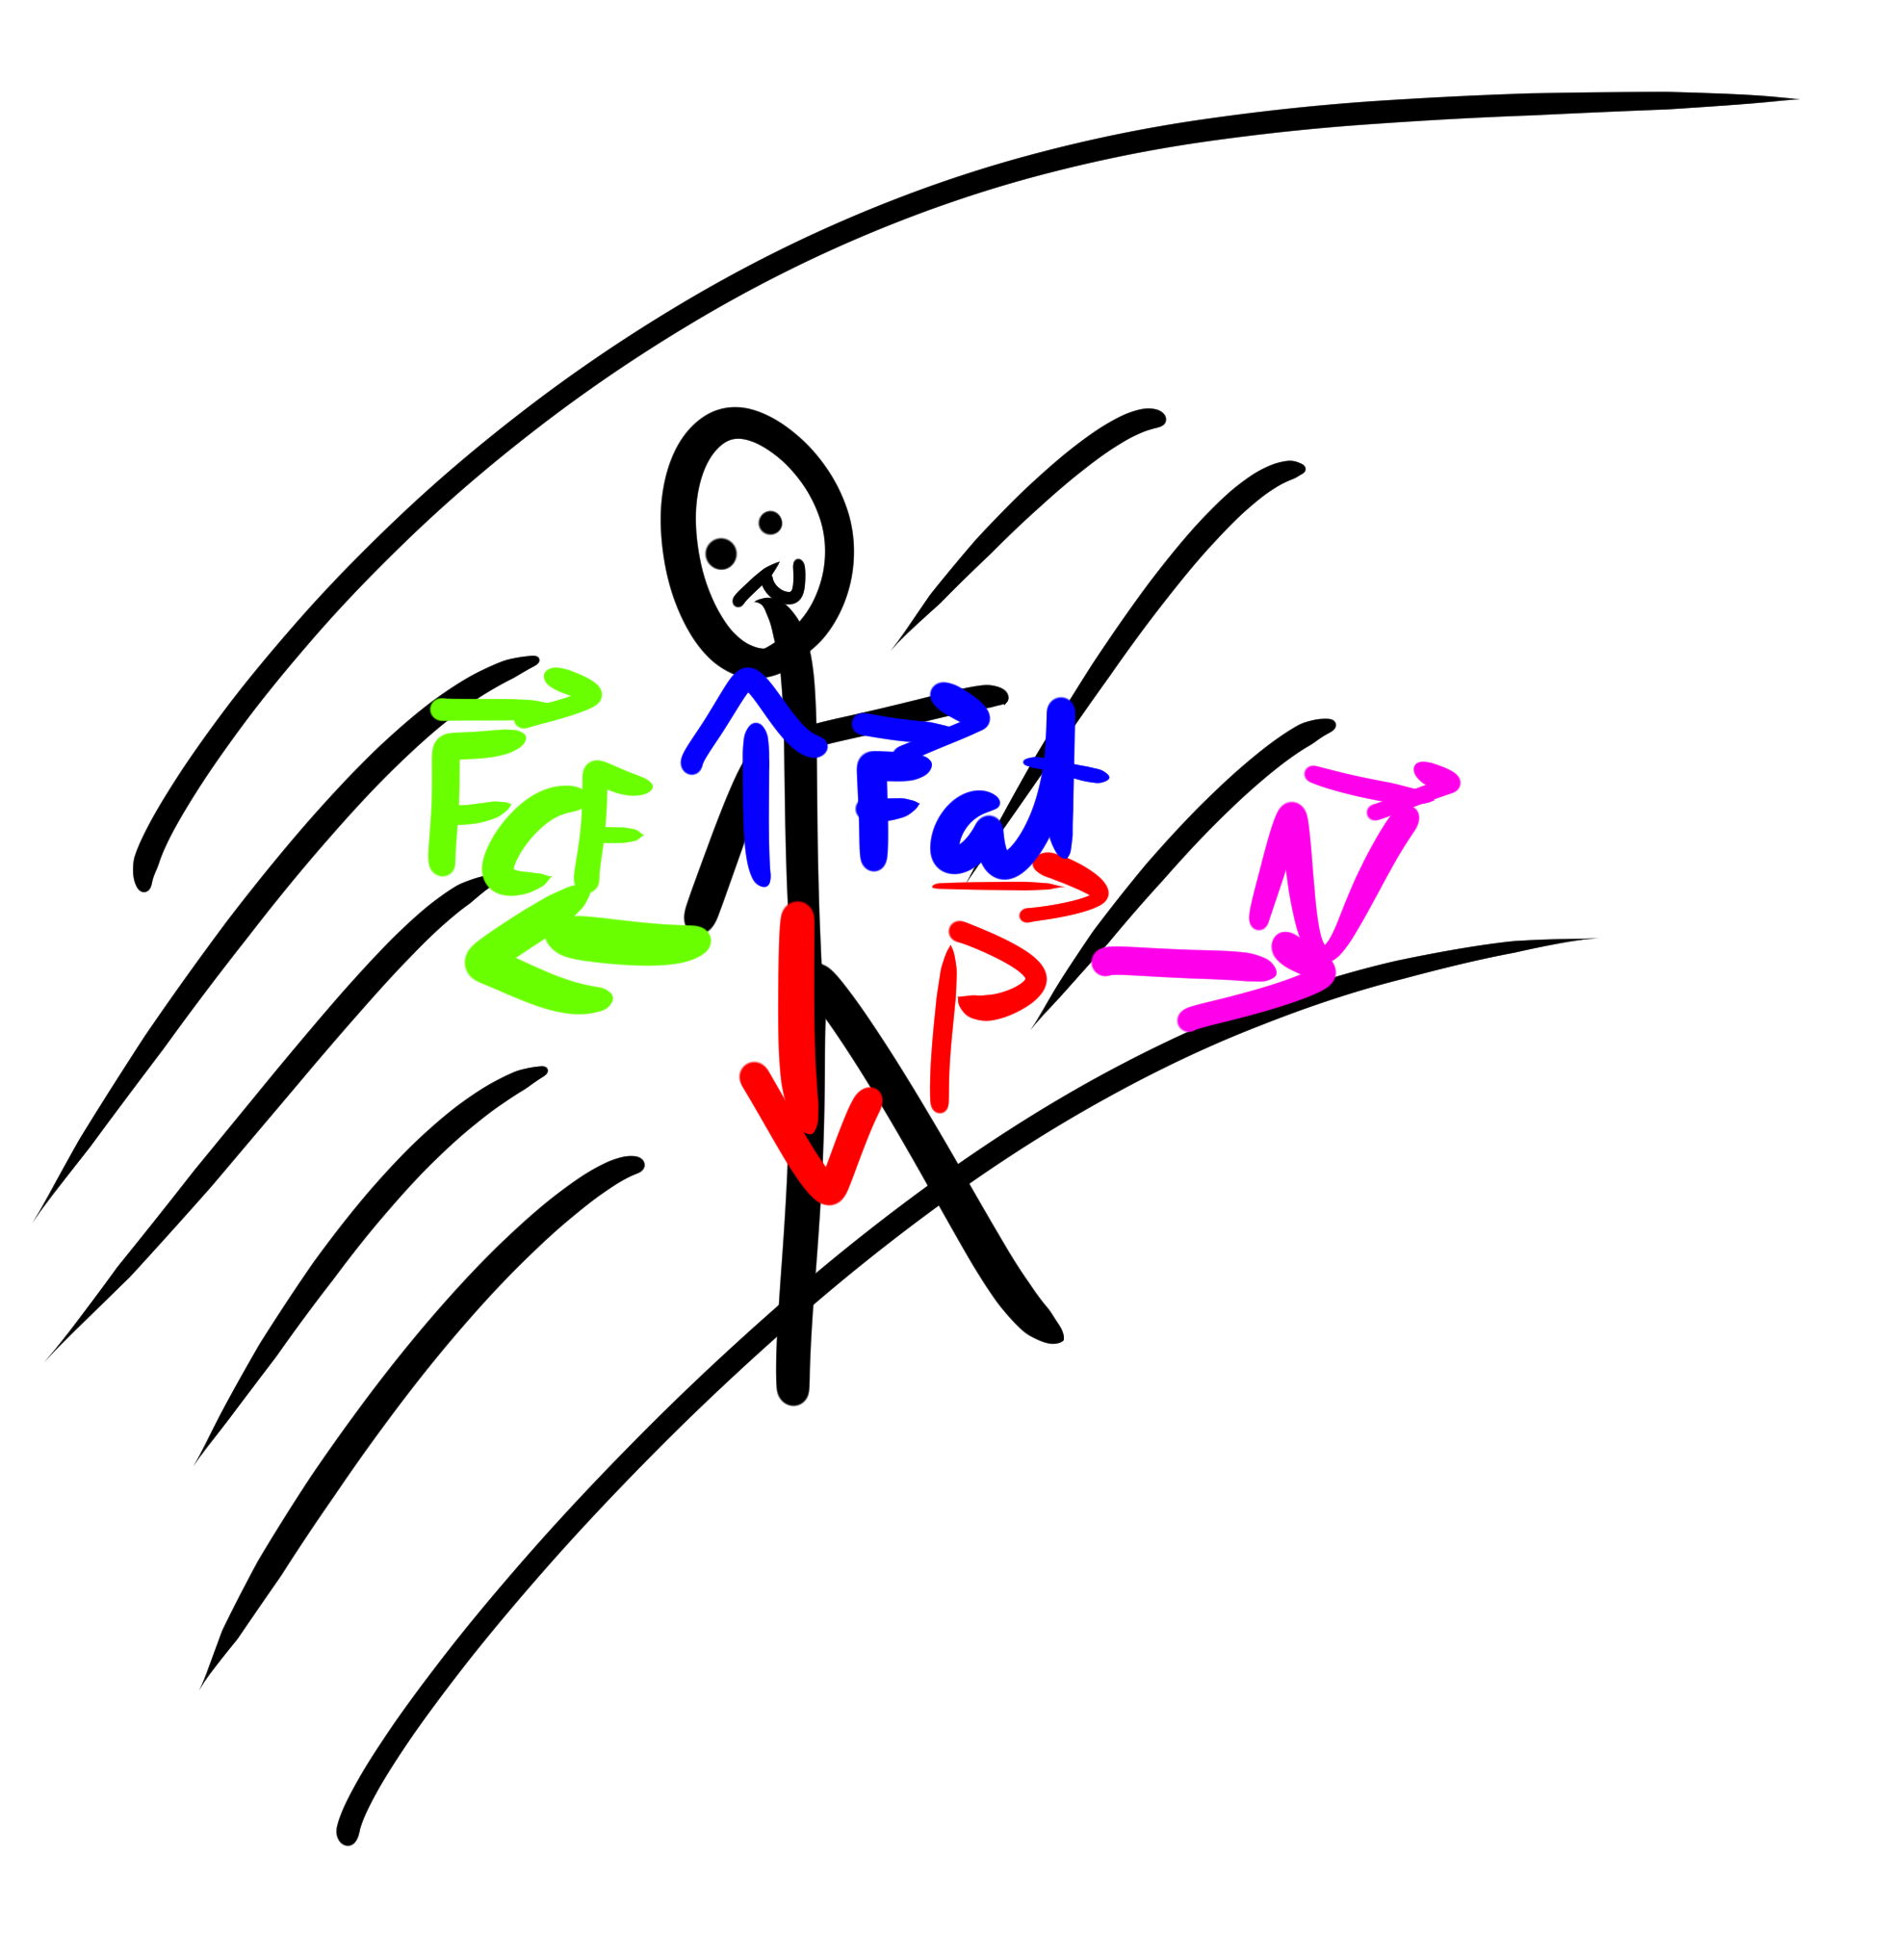
\includegraphics[width=1\linewidth]{fig4}

			\nextcol

			Adotando o referencial acelerado, temos uma força fictícia (centrífuga) $ \vec{F_{cf}} $ que pressiona o indivíduo na parede do cilindro. Além dessa, temos $\vec{N}$ que é a reação normal do cilindro no indivíduo, o peso $ \vec{P} $ e a força de atrito para cima, que o mantém estático verticalmente.

			Para que o indivíduo permaneça ``grudado'' na parede do cilindro, devemos ter o módulo do peso igualando o módulo da força de atrito para que este não caia, portanto
			\begin{equation}\label{eq:MgFat}
				|\vec{P}|=|\vec{F_{at}}|\implies M\,g=\mu\,|\vec{N}|,
			\end{equation}
			onde $ g $ é o módulo da aceleração da gravidade.

			Como o indivíduo se move numa trajetória circular, sabemos que a normal tem a forma de uma força centrípeta, dessa forma, substituímos $ |\vec{N}|=M\,\omega^{2}\,R $ em \ref{eq:MgFat}:
			\begin{equation}\label{eq:omegaMin}
				M\,g=\mu\,M\,\omega^{2}\,R\implies \omega = \sqrt{\dfrac{g}{\mu\,R}}
			\end{equation}
			que é a velocidade angular mínima para que o indivíduo não caia.

		\end{multi}

		\begin{unindent}
			\item Estimando uma capacidade de 60 pessoas, cada qual tomando \SI{0.7}{\meter} (largura de uma porta comum), temos
			\[ \dfrac{2\pi\,R}{\num{0.7}}=60\implies R\approx \SI{6.68}{\meter} \]

			Adotando $ g=\SI{9.81}{\meter\per\second\squared}, \mu=\num{0.7} $ e $ \pi=\num{3.14} $, temos
			\[ f=\dfrac{1}{T}=\dfrac{\omega}{2\pi}=\dfrac{\sqrt{\num{9.81}/(\num{0.7}\cdot\num{6.68})}}{2\cdot\num{3.14}}\approx \SI{0.23}{\hertz}  \]
		\end{unindent}

	\end{solution}



	\question Uma corda de densidade uniforme, massa total $ M $ e comprimento $ L $ presa em uma das extremidades roda com velocidade angular constante $ \omega $ em um movimento horizontal segundo a Fig. \ref{fig:fig1}. Desconsidere a força gravitacional.

	\begin{figure}[H]
		\centering
		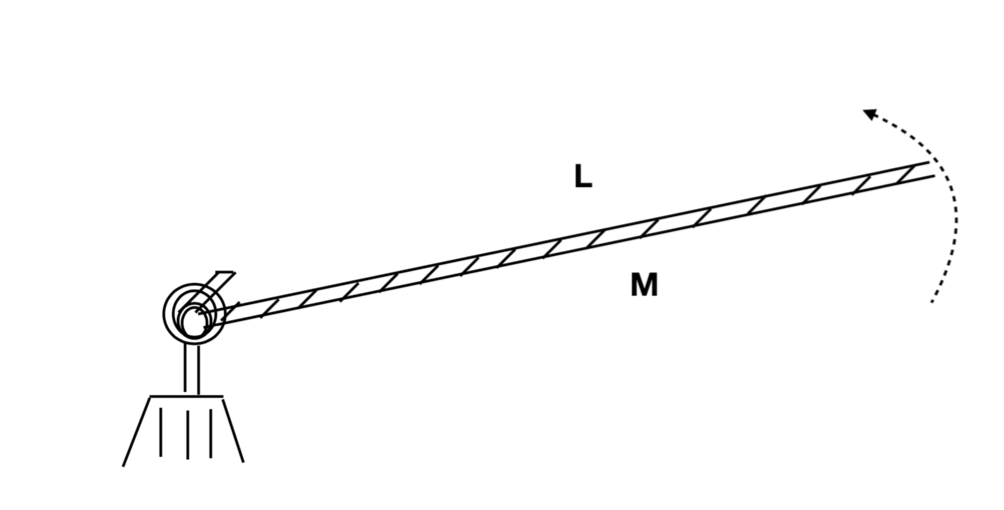
\includegraphics[width=0.7\linewidth]{screenshot001}
		\caption{Corda girando com velocidade angular $ \omega $.}
		\label{fig:fig1}
	\end{figure}

	\begin{enumerate}
		\item Considere uma porção da corda entre os pontos $ r $ e $ r + \Delta r $. Qual a massa dessa porção?
		\item Escreva a equação de movimento para a porção da corda do item 1.
		\item Tome o limite de $ \Delta r \to 0 $ para encontrar uma equação diferencial.
		\item Resolva a equação diferencial para encontrar $ T(r) $. Lembre-se que uma das extremidades da corda está livre!
	\end{enumerate}

	\begin{solution}
		\begin{unindent}[start=1]
			\item Como a densidade da corda $ \rho $ é uniforme, $ \rho=M/L=m/\Delta r $, onde $ m $ é uma porção de massa no trecho $ r\to r+\Delta r $. Dessa forma, $ m=M\,\Delta r/L $.

			\item Sendo a tensão da corda num ponto $ r $ dada por $ T(r) $, pela segunda lei de Newton sabemos que
			\begin{equation}\label{eq:deltaT}
				T(r+\Delta r)-T(r)=\Delta T=m\,a_{cp},
			\end{equation}
			onde $ a_{cp} $ é a aceleração centrípeta do trecho. Isso se dá pois a corda executa um movimento rotacional em toda a sua extensão.

			\item Tomando o limite de $ \Delta r\to0 $, temos
			\begin{align}
				\lim\limits_{\Delta r\to 0}\Delta T=\dif T & =\dif m\,a_{cp}\nonumber                           \\
				\intertext{dessa forma, $ \dif m=M\,\dif r/L $ e $ a_{cp}=-\omega^{2}r $ (veja a nota%
				\footnote{Repare que, no limite $ \Delta r\to 0 $, a diferença na aceleração em $ r $ e $ r+\dif r $ torna-se desprezível: sejam $ a_{cp}=-\omega^{2}\del{r+\dif r} $ e $ a_{cp}'=-\omega^{2}\,r $, tomando o produto $ \dif m\,a_{cp}=-(M/L)\dif r\,\omega^{2}\del{r+\dif r}=-(M/L)\omega^{2}\del[1]{r\,\dif r+\cancelto{0}{\dif r^{2}}}=-(M/L)\omega^{2}\,r\,\dif r=\dif m\,a_{cp}' $. $ \blacklozenge $ \ (Kleppner, p. 96)}%
				). Substituindo, temos}
				\dif T                                     & =-\dfrac{M}{L}\omega^{2}\,r\,\dif r\label{eq:difT}
			\end{align}
			%		\end{unindent}
			%	\end{solution}
			%
			%	\begin{solution}
			%		\begin{unindent}
			\item Resolvendo \ref{eq:difT}, temos:
			\begin{align*}
				\int_{T(0)}^{T(r)}\dif T & =\int_{0}^{r}-\dfrac{M}{L}\omega^{2}\,r'\,\dif r'               \\
				T(r)-T(0)                & =-\dfrac{M}{L}\omega^{2}\eval{\del{\dfrac{1}{2}r'^{2}}}_{0}^{r} \\
				T(r)                     & =T(0)-\dfrac{M\,\omega^{2}\,r^{2}}{2L}
			\end{align*}
			Sabendo que a extremidade da corda está livre, $ T(L)=0 $, portanto:
			\[ T(L)=0\implies T(0)=\dfrac{M\,\omega^{2}\,L}{2} \]
			Dessa forma, temos
			\[ T(r)=\dfrac{M\,\omega^{2}}{2L}\del{L^{2}-r^{2}} \]
		\end{unindent}
	\end{solution}



	\question Uma mesa com atrito desprezível tem um furo no seu centro como na Fig. \ref{fig:fig2}. Um bloco $ A $ sobre a mesa está conectado por um fio a um bloco $ B $ pendurado pelo fio que passa pelo furo do centro da mesa. O fio tem comprimento $\ell$ e massa desprezível. Inicialmente $ B $ está parado e $ A $ rodando desenvolvendo uma trajetória circular de raio constante $ r_0 $ e velocidade angular uniforme $ \omega_0 $. $ B $ é solto em $ t = 0 $.

	\begin{figure}[H]
		\centering
		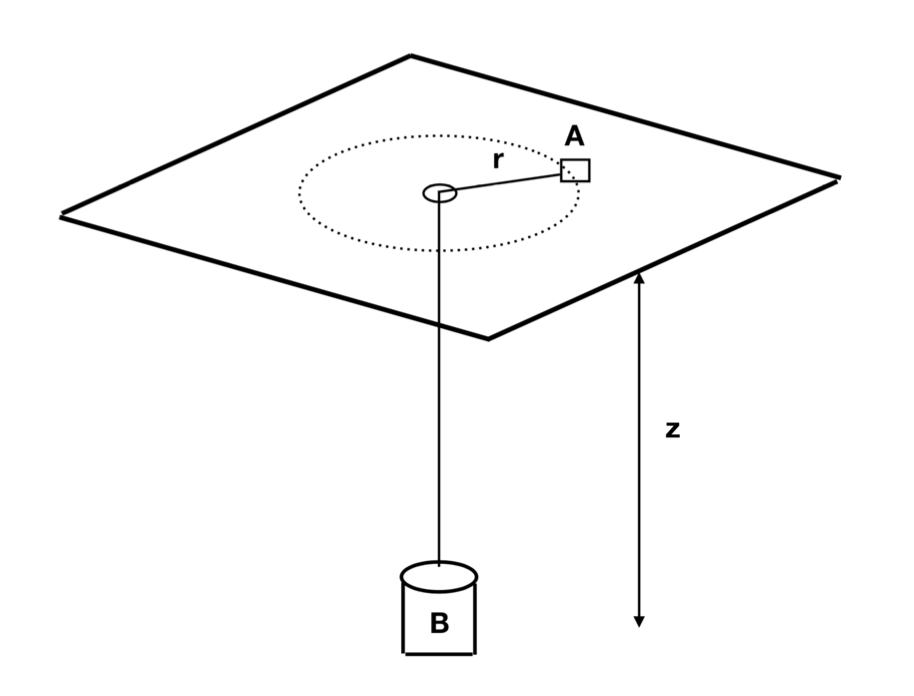
\includegraphics[width=0.5\linewidth]{screenshot002}
		\caption{Mesa com um furo no centro.}
		\label{fig:fig2}
	\end{figure}

	\begin{enumerate}
		\item Desenhe os diagramas de forças para os blocos $ A $ e $ B $.
		\item Escreva as equações de movimento para os blocos $ A $ e $ B $.
		\item Determine a aceleração do bloco $ B $ imediatamente após ser liberado em $ t = 0 $.
		\item O bloco $ B $ pode subir depois de liberado? Em que condições?
	\end{enumerate}

	\begin{solution}

		\begin{multi}
			\begin{unindent}[start=1]
				\item
			\end{unindent}

			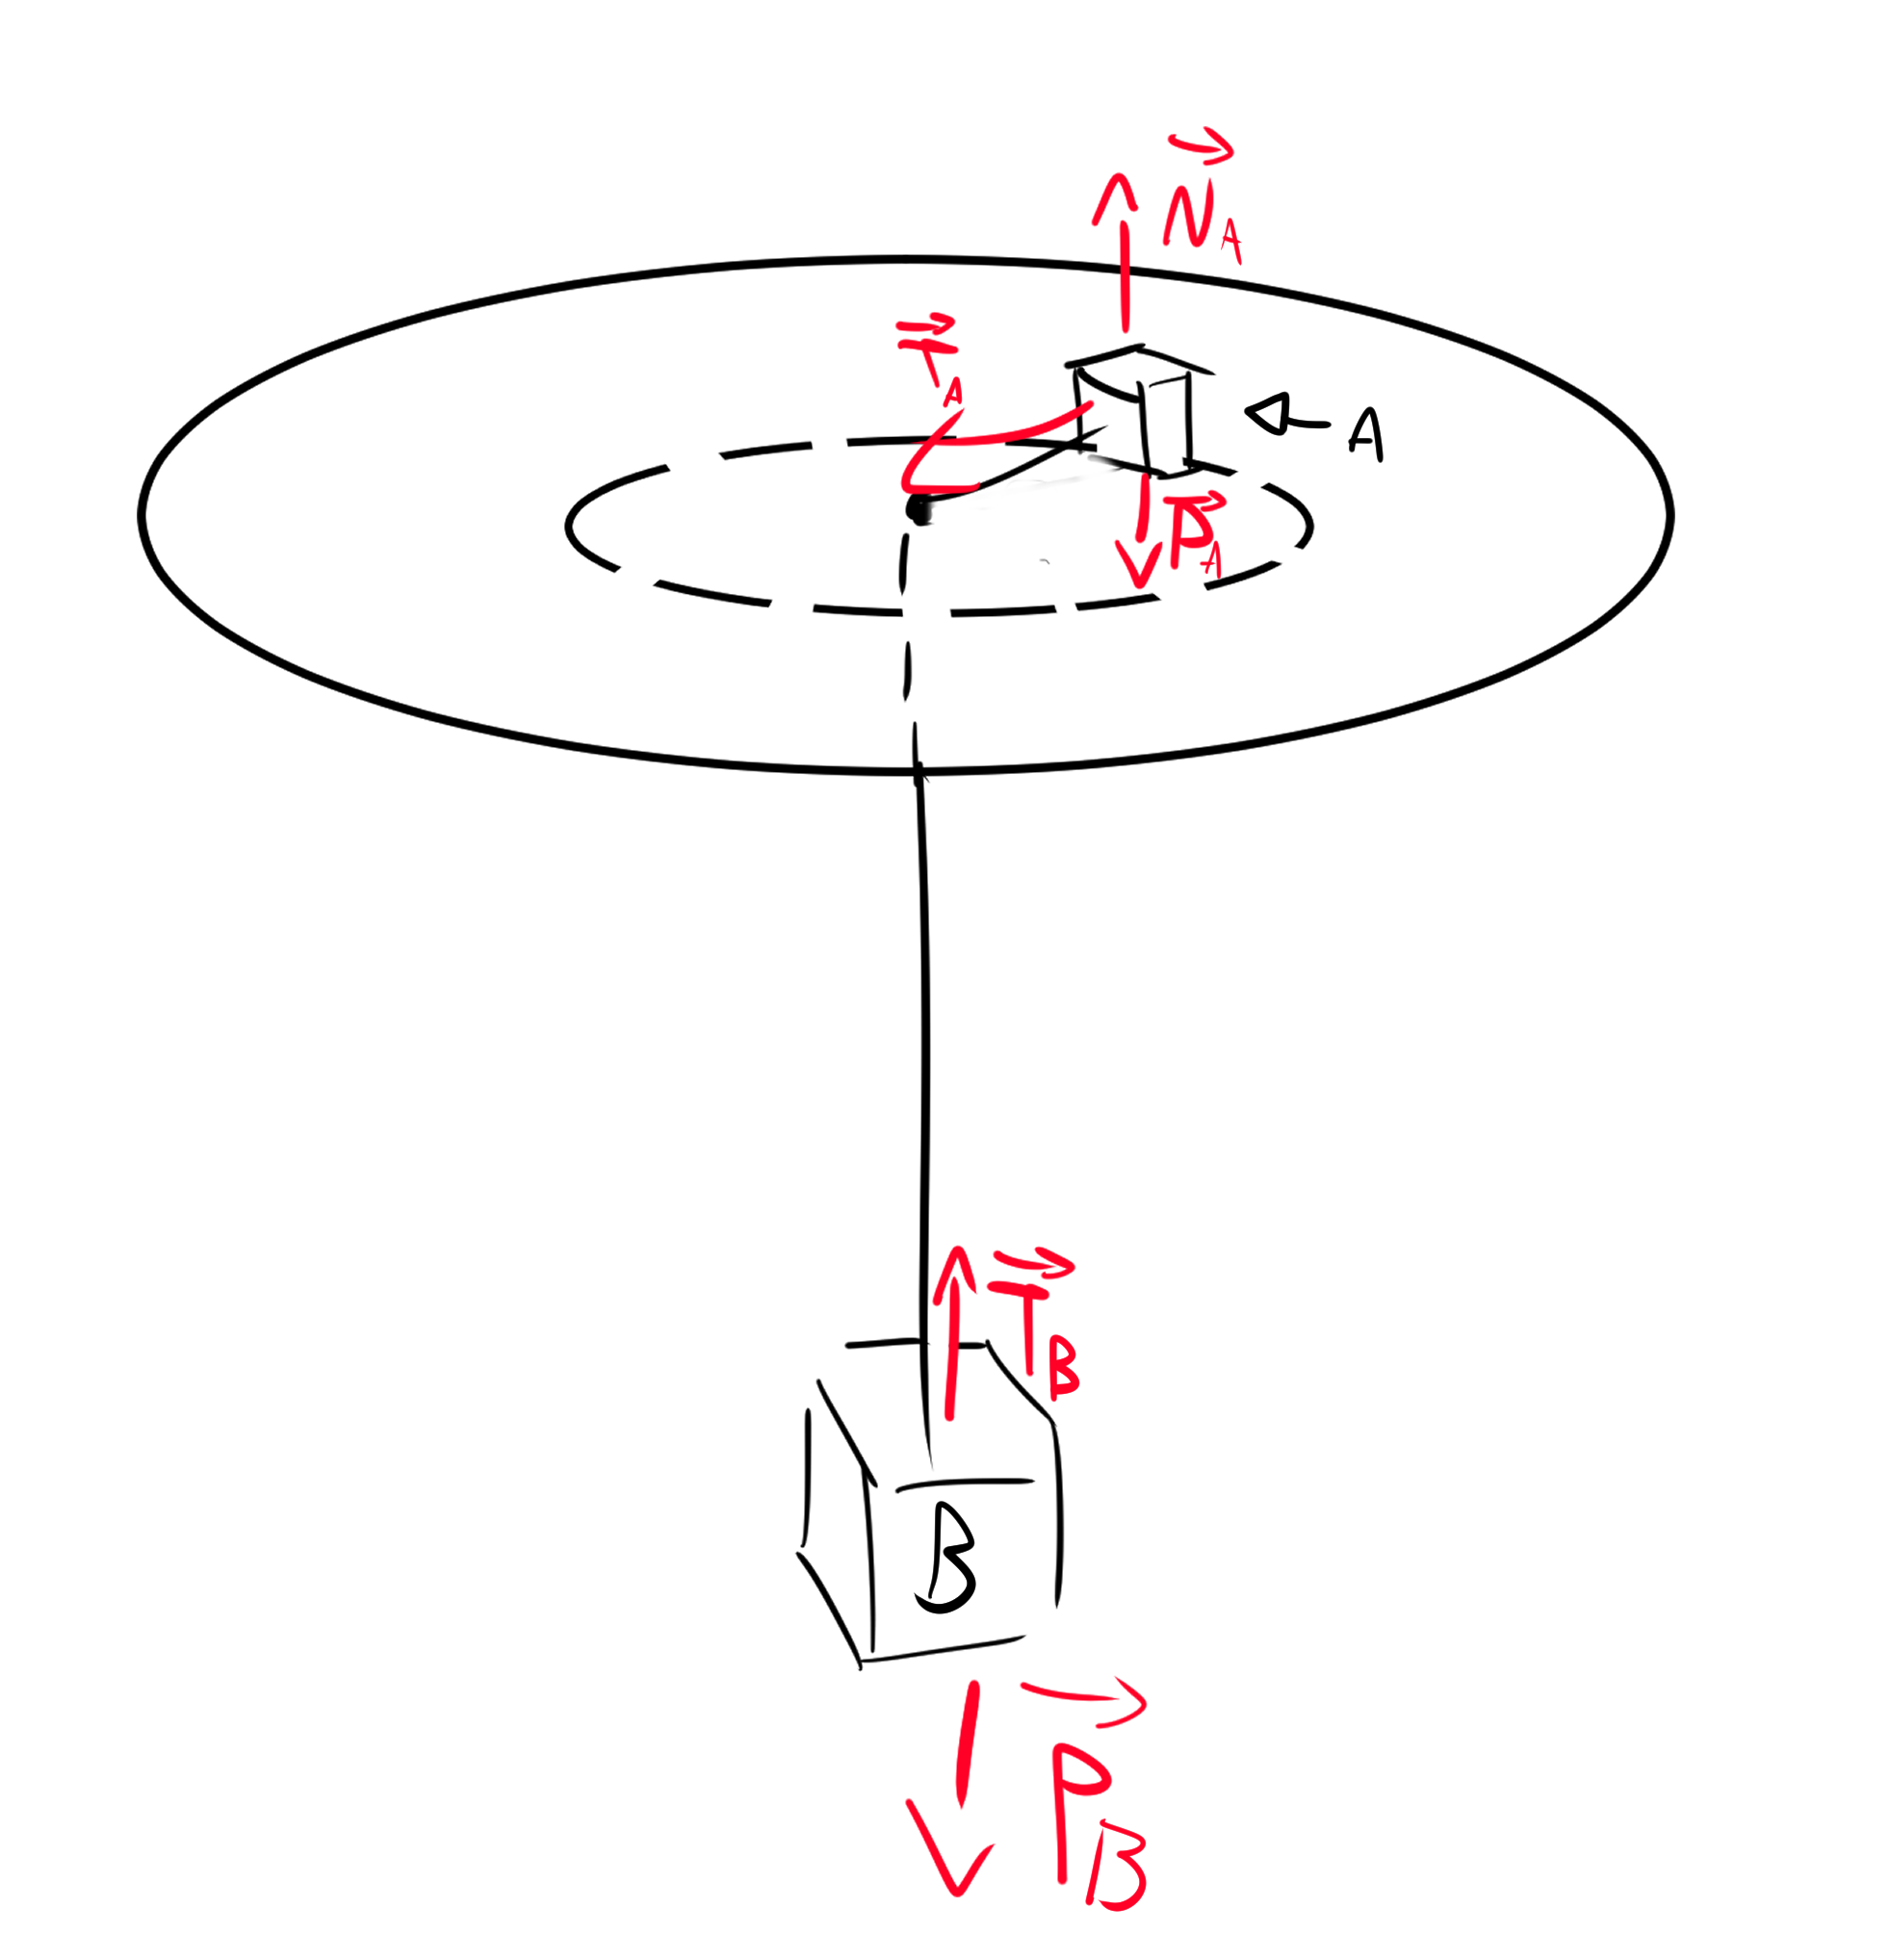
\includegraphics[width=1\linewidth]{fig5}

			\nextcol

			\begin{unindent}
				\item Definindo a origem no furo da mesa, o sentido positivo como para baixo no eixo vertical, e o vetor $ \rhat $ apontando para fora do bloco $ A $, que gira.

				Sejam $ m_i $ a massa dos blocos $ i\in\set{A,B} $, $ \vec{P_i} $ o peso deles, $ \vec{a_i} $ sua aceleração, $ \vec{T} $ a tensão do fio atuando em ambos e $\vec{N_A}$ a normal da mesa sobre $ A $. Pela segunda lei de Newton, temos
				\begin{gather}
					\vec{P_B}+\vec{T_B}=m_B\,\vec{a_B}\label{eq:PTmbvec}\\
					\vec{P_A}+\vec{N_A}+\vec{T_A}=m_A\,\vec{a_A}\label{eq:Tmavec}
				\end{gather}

				\item Adotemos a notação do módulo de um vetor qualquer $ |\vec{v}|=v $. Sendo $ \vec{r} $ o vetor posição do bloco $ A $ e $ \vec{z} $ o vetor posição do bloco $ B $, temos:
				\begin{gather*}
					\vec{a_A}=\ddot{\vec{r}}=\del{\ddot{r}-r\,\dot{\theta}}\rhat+\del{r\,\ddot{\theta}+2\dot{r}\,\dot{\theta}}\that\\
					\vec{a_B}=\ddot{\vec{z}}
				\end{gather*}
			\end{unindent}

		\end{multi}


		Dessa forma, podemos escrever o módulo de \ref{eq:PTmbvec} como
		\begin{equation}\label{eq:modaccB}
			|\vec{P_B}+\vec{T_B}|=P_B-T=m_B\,\ddot{z},
		\end{equation}
		igualmente, o módulo de \ref{eq:Tmavec} pode ser escrito como
		\begin{gather}
			|\vec{T_A}|=-T=m_A\del{\ddot{r}-r\,\dot{\theta}^{2}},\label{eq:modaccAr}\\
			|\vec{P_A}+\vec{N_A}|=0=m_A\del{r\,\ddot{\theta}+2\dot{r}\,\dot{\theta}}.\label{eq:modaccAt}
		\end{gather}
		\paragraph{Nota:} $ T=|\vec{T_A}|=|\vec{T_B}| $.

		Subtraindo \ref{eq:modaccAr} de \ref{eq:modaccB}, temos
		\[ P_B=m_B\,\ddot{z}-m_A\del{\ddot{r}-r\,\dot{\theta}^{2}} \]
		e, como $ r+z=\ell\implies \ddot{z}=-\ddot{r} $
		\begin{align}
			P_B      & =m_B\,\ddot{z}+m_A\del{\ddot{z}+r\,\dot{\theta}^{2}}\nonumber   \\
			\intertext{isolando $ \ddot{z} $ ficamos com}
			\ddot{z} & =\dfrac{P_B-m_A\,r\,\dot{\theta}^{2}}{m_B+m_A}.\label{eq:ddotz}
		\end{align}
		Sendo $ P_B=m_B\,g $ ($ g $ é o módulo da aceleração da gravidade) e $ r=r_0,\dot{\theta}=\omega_0 $ no momento inicial, temos
		\[ \ddot{z}=\dfrac{m_B\,g-m_A\,r_0\,\omega_0^{2}}{m_B+m_A} \]
		\begin{unindent}

			\item Caso $ \ddot{z}<0 $, o bloco $ B $ subirá, dessa forma, pela equação \ref{eq:ddotz}, temos
			\[ \ddot{z}<0\implies \underbrace{m_A\,r\,\dot{\theta}^{2}}_{=\,F_{cp}}>P_B \]
			onde $ F_{cp} $ é a força centrípeta.
		\end{unindent}
	\end{solution}



	\question O pêndulo cônico é um sistema no qual um pêndulo é posto em movimento na direção tangente à uma circunferência, de acordo com a Fig. \ref{fig:fig3}. Supondo que o movimento seja circular uniforme com velocidade $ v_0 $, determine:

	\begin{figure}[H]
		\centering
		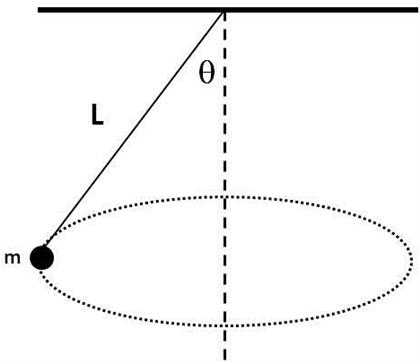
\includegraphics[width=0.4\linewidth]{screenshot003}
		\caption{Pêndulo cônico.}
		\label{fig:fig3}
	\end{figure}

	\begin{parts}
		\part o ângulo $ \theta $;

		\begin{solution}
			Sendo as forças no sistema o peso $ \vec{P} $ da massa $ m $ e $ \vec{T} $ a tensão na corda, pela segunda lei de Newton, temos:
			\useshortskip
			\begin{equation}\label{eq:PTma}
				\vec{P}+\vec{T}=m\,\vec{a}
			\end{equation}
			onde $ \vec{a} $ é a aceleração da massa.

			Adotemos a notação $ |\vec{v}|=v $, e o sentido positivo como para cima na vertical, e para o centro na horizontal ($ \rhat $).

			Dessa forma, tomando o módulo de \ref{eq:PTma}, temos
			\useshortskip
			\begin{gather}
				|\vec{P}+\vec{T}|=-P+T\cos\theta=0\label{eq:PTmav}\\
				T\sin\theta=m\,a_{cp}\label{eq:PTmah}
			\end{gather}
			onde $ a_{cp} $ é a aceleração centrípeta.

			Sendo $ T=P/\cos\theta $ (de \ref{eq:PTmav}), e sabendo que o raio do movimento circular é $ r=L\sin\theta $, de \ref{eq:PTmah} temos
			\useshortskip
			\begin{align*}
				\dfrac{P}{\cos\theta}\sin\theta & =m\,\omega^{2}\,L\sin\theta            \\[-0.5em]
				\cos\theta                      & =\dfrac{\omega^{2}\,L}{g}              \\[-1em]
				\theta                          & =\arccos\del{\dfrac{\omega^{2}\,L}{g}}
			\end{align*}

		\end{solution}

		\part quanto vale o trabalho feito no sistema? Você espera que a energia cinética seja conservada na ausência de atrito com o ar?

		\begin{solution}
			Supondo a ausência de forças dissipativas, a energia é conservada no sistema. E como não há mudança de energia cinética ou potencial não há trabalho realizado no sistema.
		\end{solution}
	\end{parts}


	\question Considere um foguete na superfície da Terra. O foguete está tentando alcançar a \textit{velocidade de escape}, ou seja, a velocidade inicial mínima que permite chegar com velocidade nula a uma distância infinita da Terra. Calcule a velocidade de escape no caso em que a velocidade inicial do foguete faça um ângulo $ \alpha $ com a linha vertical.

	\begin{solution}

		\begin{multi}
			Para encontrar a velocidade de escape, denotada por $ v_{esc} $, podemos utilizar o teorema trabalho-energia, considerando o trabalho realizado pela força gravitacional $ \vec{F_g} $, que é dado pela expressão
			\begin{equation}\label{eq:gfwork}
				W_{\vec{F_g}}=\int_{r_0}^{r}\vec{F_g}(r)\cdot\dif\vec{r}.
			\end{equation}

			Sendo a força gravitacional dada por
			\begin{equation}\label{eq:gforce}
				\vec{F_g}=-G\dfrac{M_T\,m}{r^{2}}\rhat
			\end{equation}
			onde $ G $ é a constante gravitacional, $ M_T $ é a massa do planeta Terra e $ r $ é a distância do corpo a partir do centro da Terra.

			Tomando o diferencial $ \dif\vec{r}=\rhat\dif r+r\that\dif\theta $ (que podemos derivar pelo rascunho da situação, ao lado), podemos tomar a integral do trabalho:

			\nextcol

			\centering
			\begin{tikzpicture}
				\draw (0,0) arc (90:85:10);
				\draw (0,0) arc (90:120:10);

				\coordinate (O) at (0,0);

				\draw[loosely dashed] (0,0) arc (10:40:8) coordinate (A) arc (40:70:8) coordinate (B);
				\draw[-Latex] (0,0) -- node[pos=0.6,inner sep=1pt,fill=white] {$ \vec{r_0} $} (A);
				\draw[-Latex] (0,0) -- node[pos=0.7,inner sep=1pt,fill=white] {$ \vec{r_1} $} (B);
				\draw[dotted] (0,0) -- +(0,4) coordinate (C);
				\draw[-Latex] (A) -- node[inner sep=1pt,fill=white] {$ \dif\vec{r} $} (B);

				\draw[-Latex,dashed,red] (A) -- node[rotate=40,above] {$ r\that\dif\theta $} ($ (O)!(A)!(B) $);
				\draw[-Latex,dashed,red] let \p1 = ($ (A)-(O)!(A)!(B) $),
				in (A) -- node[right] {$ \rhat\dif r $} ($ (B)+(\x1,\y1) $);


				\pic[draw=black, angle radius=40pt,angle eccentricity=1,"$ \dif\theta $" {xshift=-4pt,yshift=6pt}] {angle=A--O--B};
				\pic[draw=black, angle radius=50pt,angle eccentricity=1,"$ \alpha $" {xshift=2pt,yshift=5pt}] {angle=C--O--A};
			\end{tikzpicture}
		\end{multi}

		\[ 	W_{\vec{F_g}}=\int_{r_0}^{r}\vec{F_g}(r)\cdot\dif\vec{r}=\int_{r_0}^{r}-G\dfrac{M_T\,m}{r^{2}}\rhat\cdot\del{\rhat\dif r+r\that\dif\theta} \]

		\begin{multi}[2][t]
			como $ \that $ é perpendicular à $ \rhat $, somente a componente $ \rhat $ permanece após a realização do produto escalar,
			\begin{align*}
				W_{\vec{F_g}} & =-G\,M_T\,m\int_{r_0}^{r}\dfrac{1}{r^{2}}\dif r \\
				\intertext{consideremos o movimento saindo da superfície da Terra, de raio $ R_T $, e indo até um ponto $ r $,}
				              & =-G\,M_T\,m\int_{R_T}^{r}r^{-2}\dif r           \\
				              & =-G\,M_T\,m\eval{\del{-r^{-1}}}_{R_T}^{r}       \\
				W_{\vec{F_g}} & =-G\,M_T\,m\del{\dfrac{1}{R_T}-\dfrac{1}{r}}
			\end{align*}
			que deve ser igual à variação de energia cinética do sistema.

			\nextcol

			Adotando a velocidade final $ v=0 $, e o ponto final $ r\to\infty $, teremos, pelo teorema trabalho-energia:
			\begin{align*}
				\lim\limits_{r\to\infty}-G\,M_T\,m\del{\dfrac{1}{R_T}-\dfrac{1}{r}} & =\cancelto{0}{\dfrac{1}{2}m\,v^{2}}-\dfrac{1}{2}m\,v_{esc}^{2} \\
				2G\,M_T\cdot\dfrac{1}{R_T}                                          & =v_{esc}^{2}                                                   \\
				v_{esc}                                                             & =\sqrt{\dfrac{2G\,M_T}{R_T}}                                   \\
				\intertext{como $ g=F_g/m=G\,M_T/R_T^{2} $, temos}
				v_{esc}                                                             & =\sqrt{2g\,R_T}
			\end{align*}
		\end{multi}


	\end{solution}

	\clearpage

	\question Considere um pêndulo simples, de comprimento $ L $ e massa $ M $. Inicialmente, o pêndulo se encontra a um ângulo $ \theta_0 $ em relação à vertical. O ângulo $ \theta_0 $ \textit{não é pequeno}.

	\begin{parts}
		\part Calcule a velocidade do pêndulo quando o ângulo com a vertical é $ \theta = 0 $ na ausência de atrito;

		\begin{solution}
			\begin{multi}
				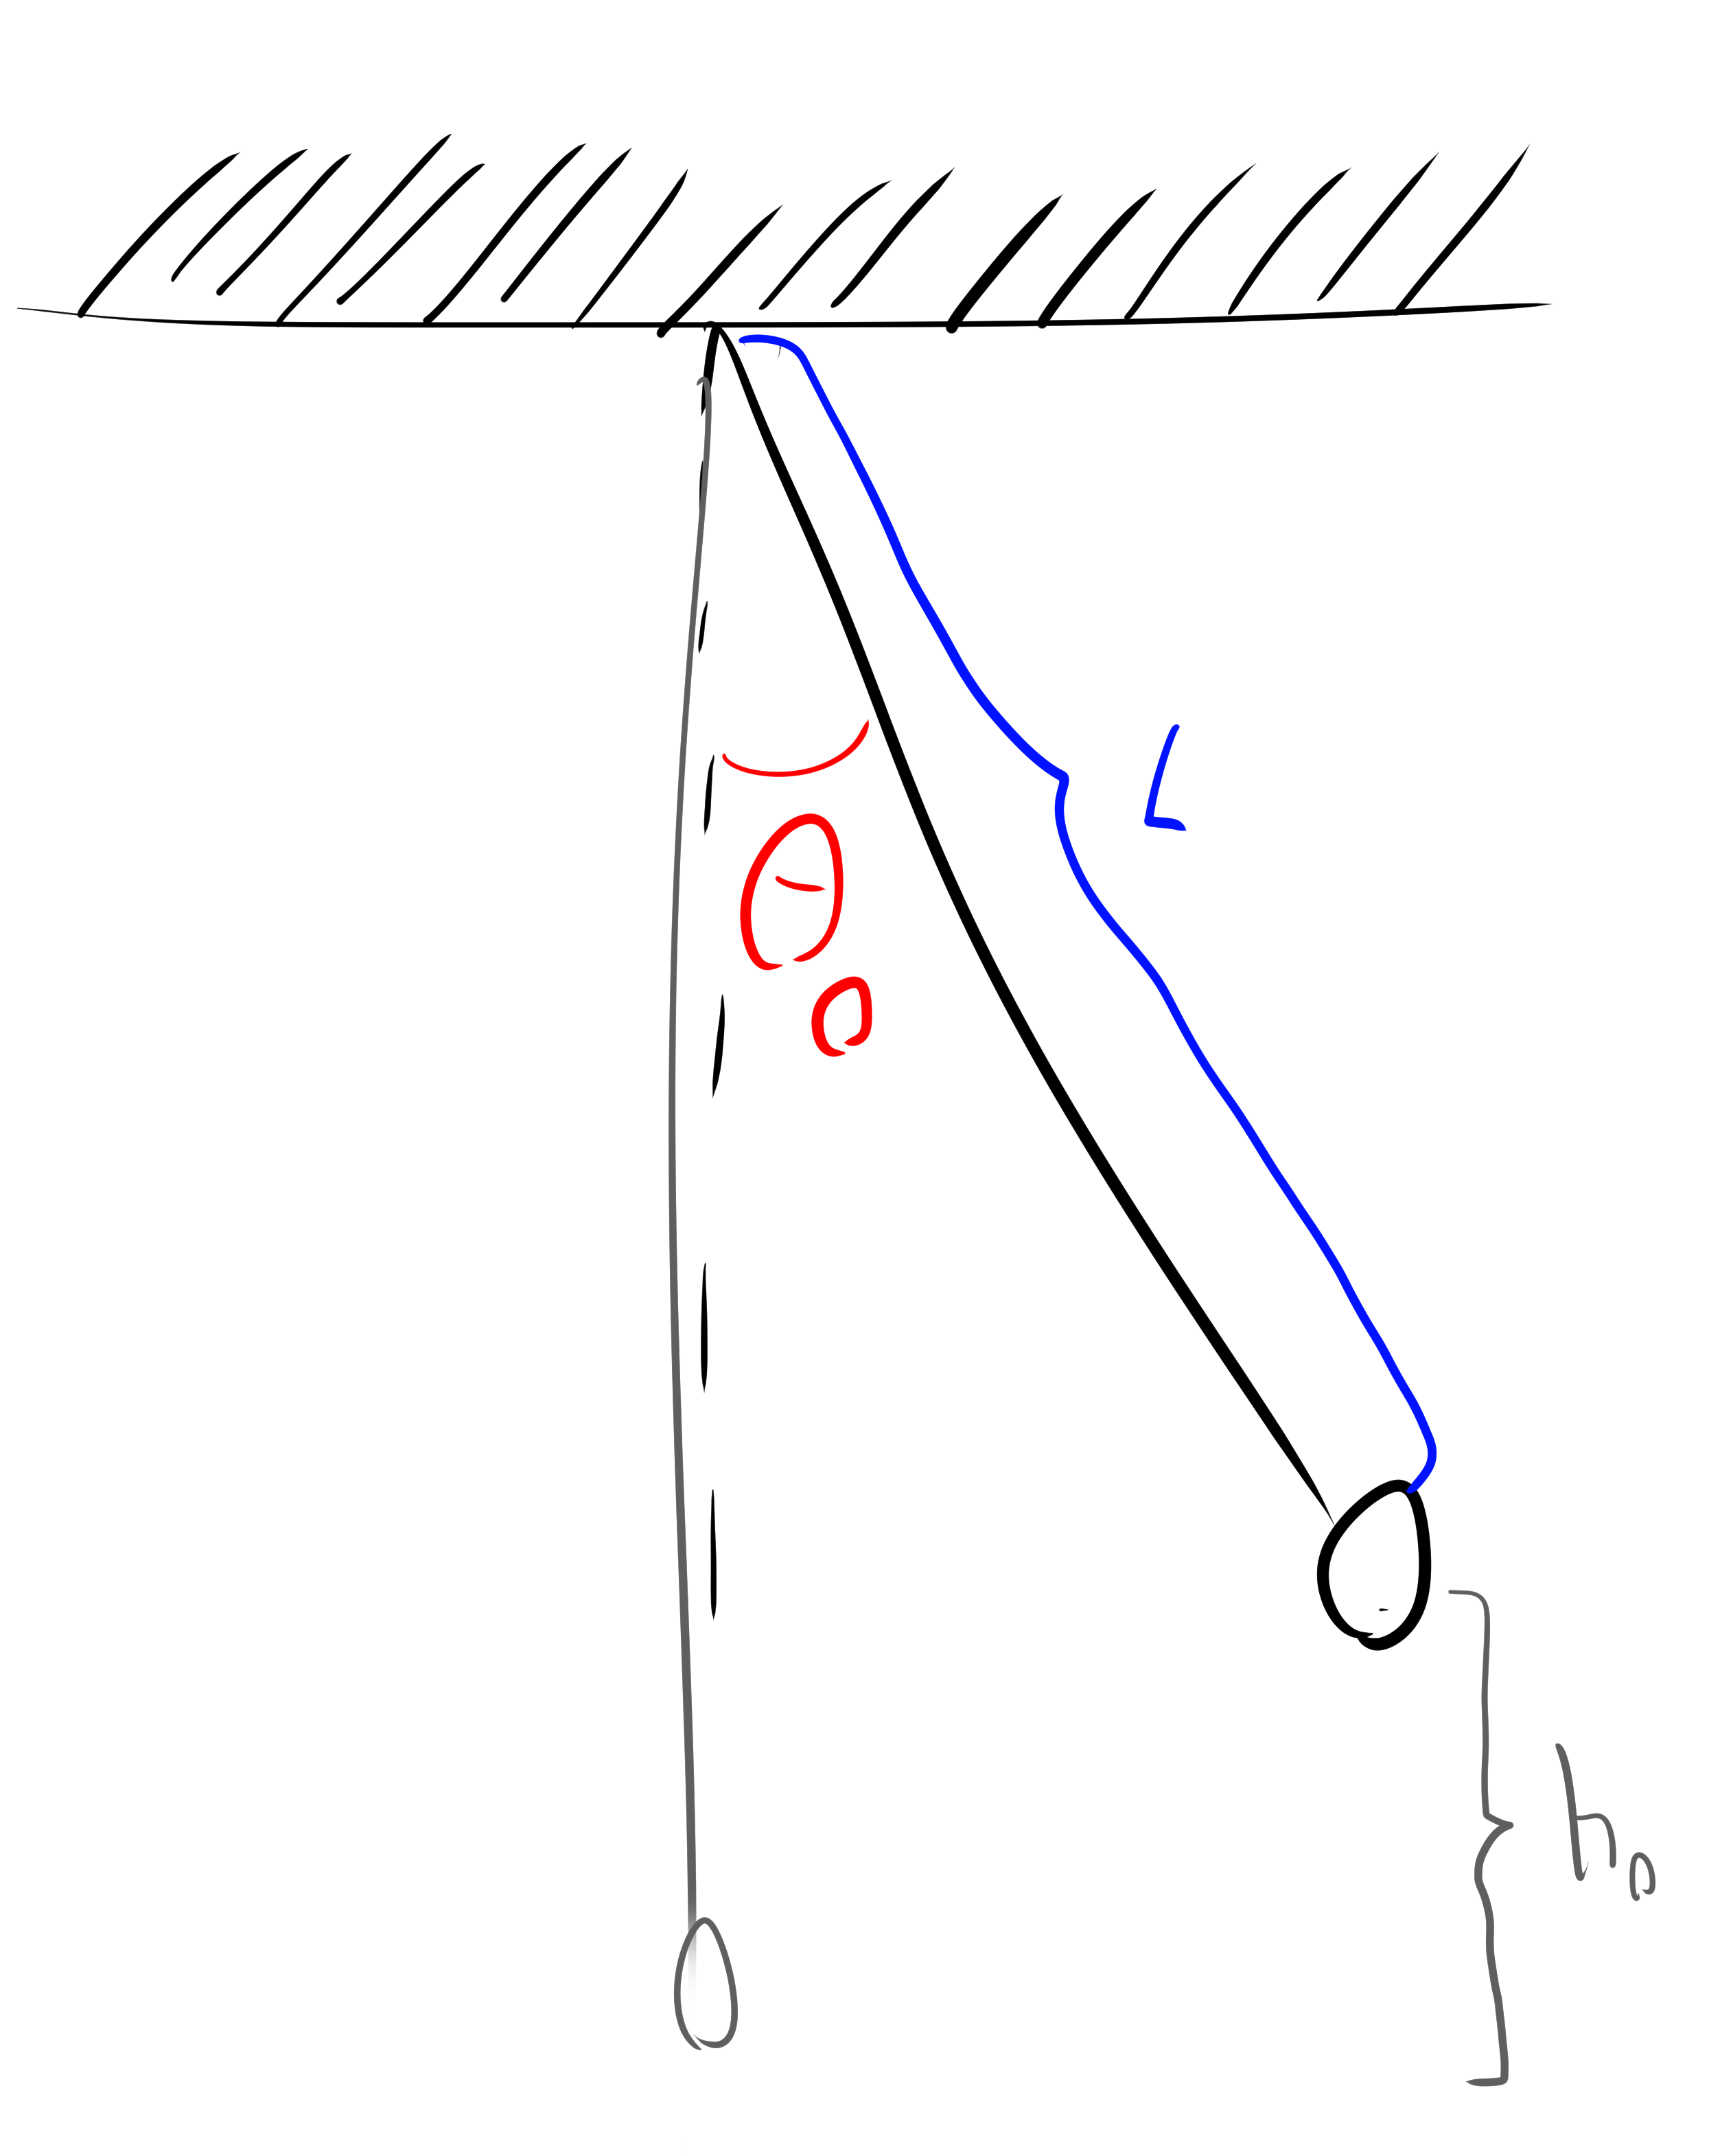
\includegraphics[width=1\linewidth]{fig6}

				\nextcol

				Considerando o sistema livre de forças dissipativas, sabemos que há conservação de energia, e, portanto
				\begin{align}
					K_0+U_0=K+U\implies \nonumber \\ \dfrac{1}{2}M\,v_0^{2}+M\,g\,h_0=\dfrac{1}{2}M\,v^{2}+M\,g\,h\label{eq:enCons}
				\end{align}
				onde o índice $ 0 $ indica que a quantidade se refere a um momento inicial.

				Adotando o referencial $ U(\theta=0)=0 $ (que é o ponto mais baixo da trajetória), e considerando que o pêndulo parte do repouso no ângulo $ \theta_0 $, de \ref{eq:enCons}, temos
				\begin{align*}
					M\,g\,h_0 & =\dfrac{1}{2}M\,v^{2}             \\
					\intertext{sabemos que $ h_0=L-L\cos\theta_0 $, portanto}
					v         & =\sqrt{2g\,L\del{1-\cos\theta_0}}
				\end{align*}
			\end{multi}
		\end{solution}

		\part Esboce o \textit{diagrama da energia} do sistema, ou seja, o gráfico da energia do pêndulo em função do ângulo $ \theta $ (sempre supondo ausência de atrito).

		\begin{solution}
			\centering
			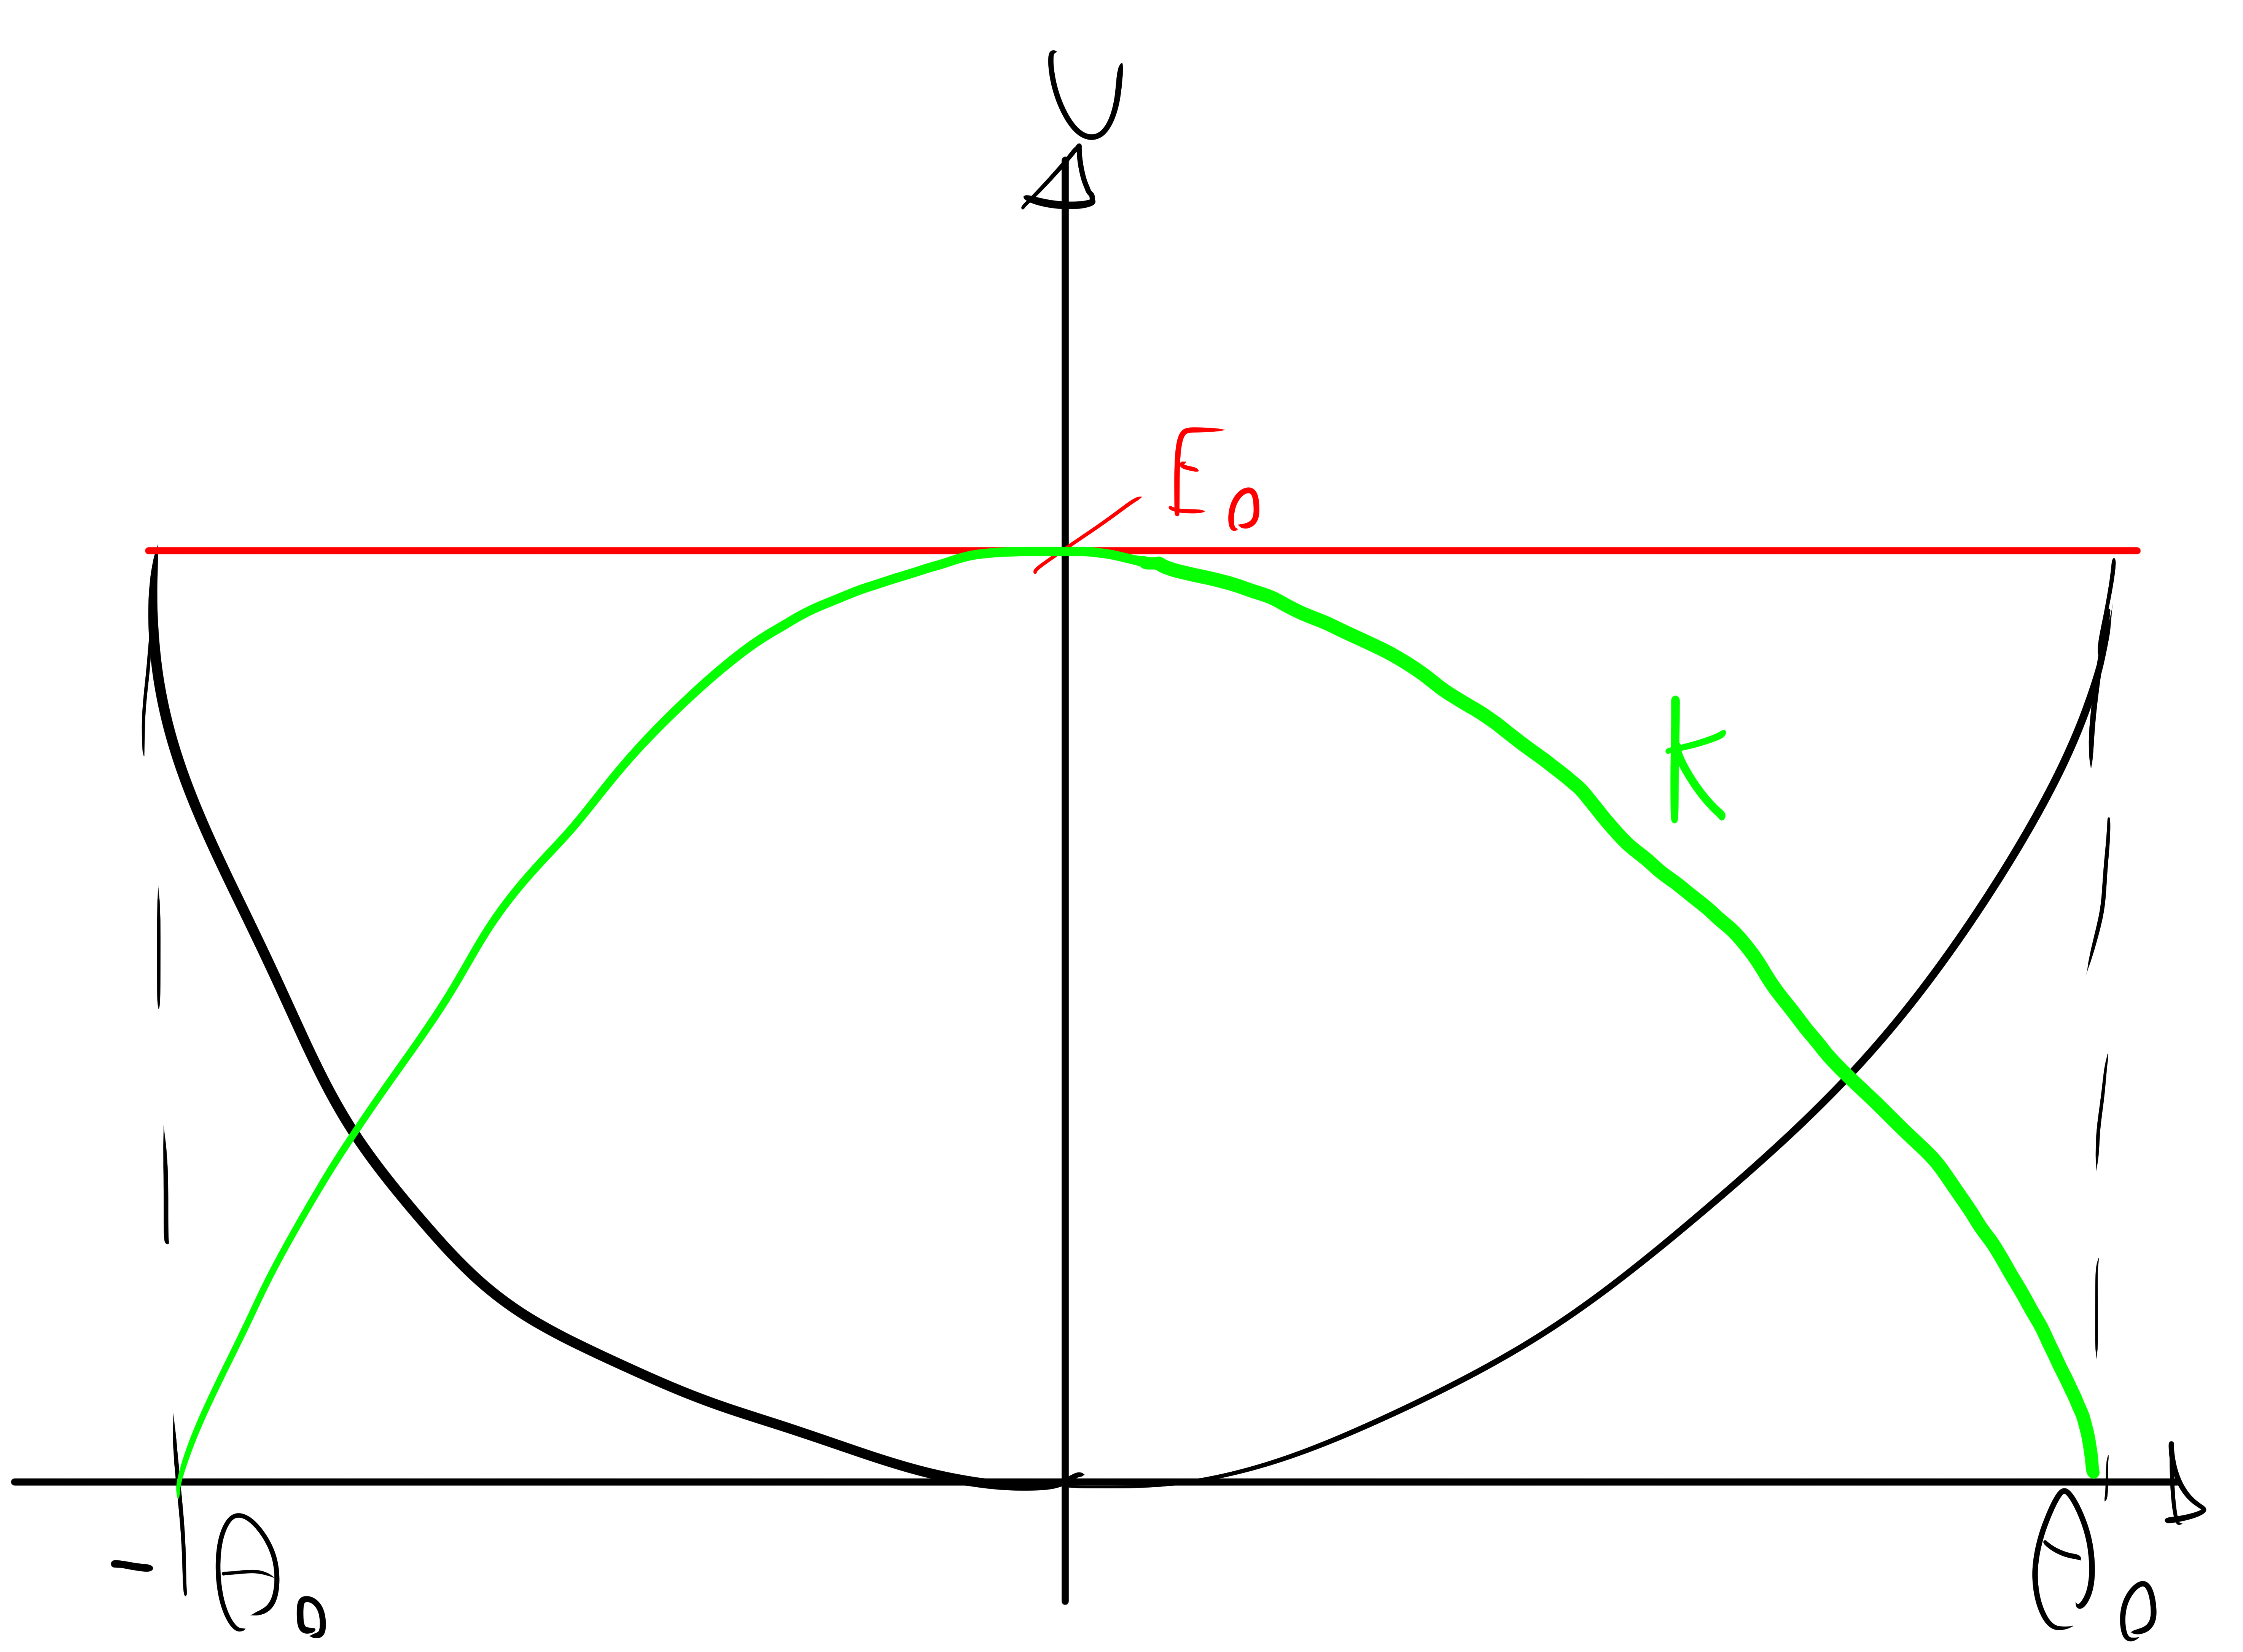
\includegraphics[width=0.5\linewidth]{fig7}
		\end{solution}
	\end{parts}

	\clearpage

	\question Considere um corpo puntiforme de massa $ m $ inicialmente no topo de uma esfera de raio $ R $ sem atrito. O corpo começa a deslizar na superfície da esfera até perder contato com a mesma. Calcule a altura do corpo no momento em que perde contato com a esfera.

	\begin{solution}

		\begin{multi}
			Aproximando a posição inicial do corpo como exatamente no topo da esfera (o que a faria ficar lá para sempre), e sabendo que o corpo executa uma trajetória contida num plano, definimos sua posição inicial como origem, no eixo horizontal a direita como sentido positivo, e, no eixo vertical, positivo para baixo.

			Definindo um ângulo $ \theta $ do corpo com uma reta horizontal que passa pelo centro da esfera, denotando valores iniciais pelo índice $ 0 $, temos, por conservação de energia\footnote{Não há forças dissipativas no sistema.}
			\begin{align}
				K_0+U_0  & =K+U\implies                     \\
				m\,g\,2R & =\dfrac{1}{2}m\,v^{2}+m\,g\,h    \\
				v^{2}    & =2g\del{2R-h}\label{eq:v2circle}
			\end{align}

			\nextcol

			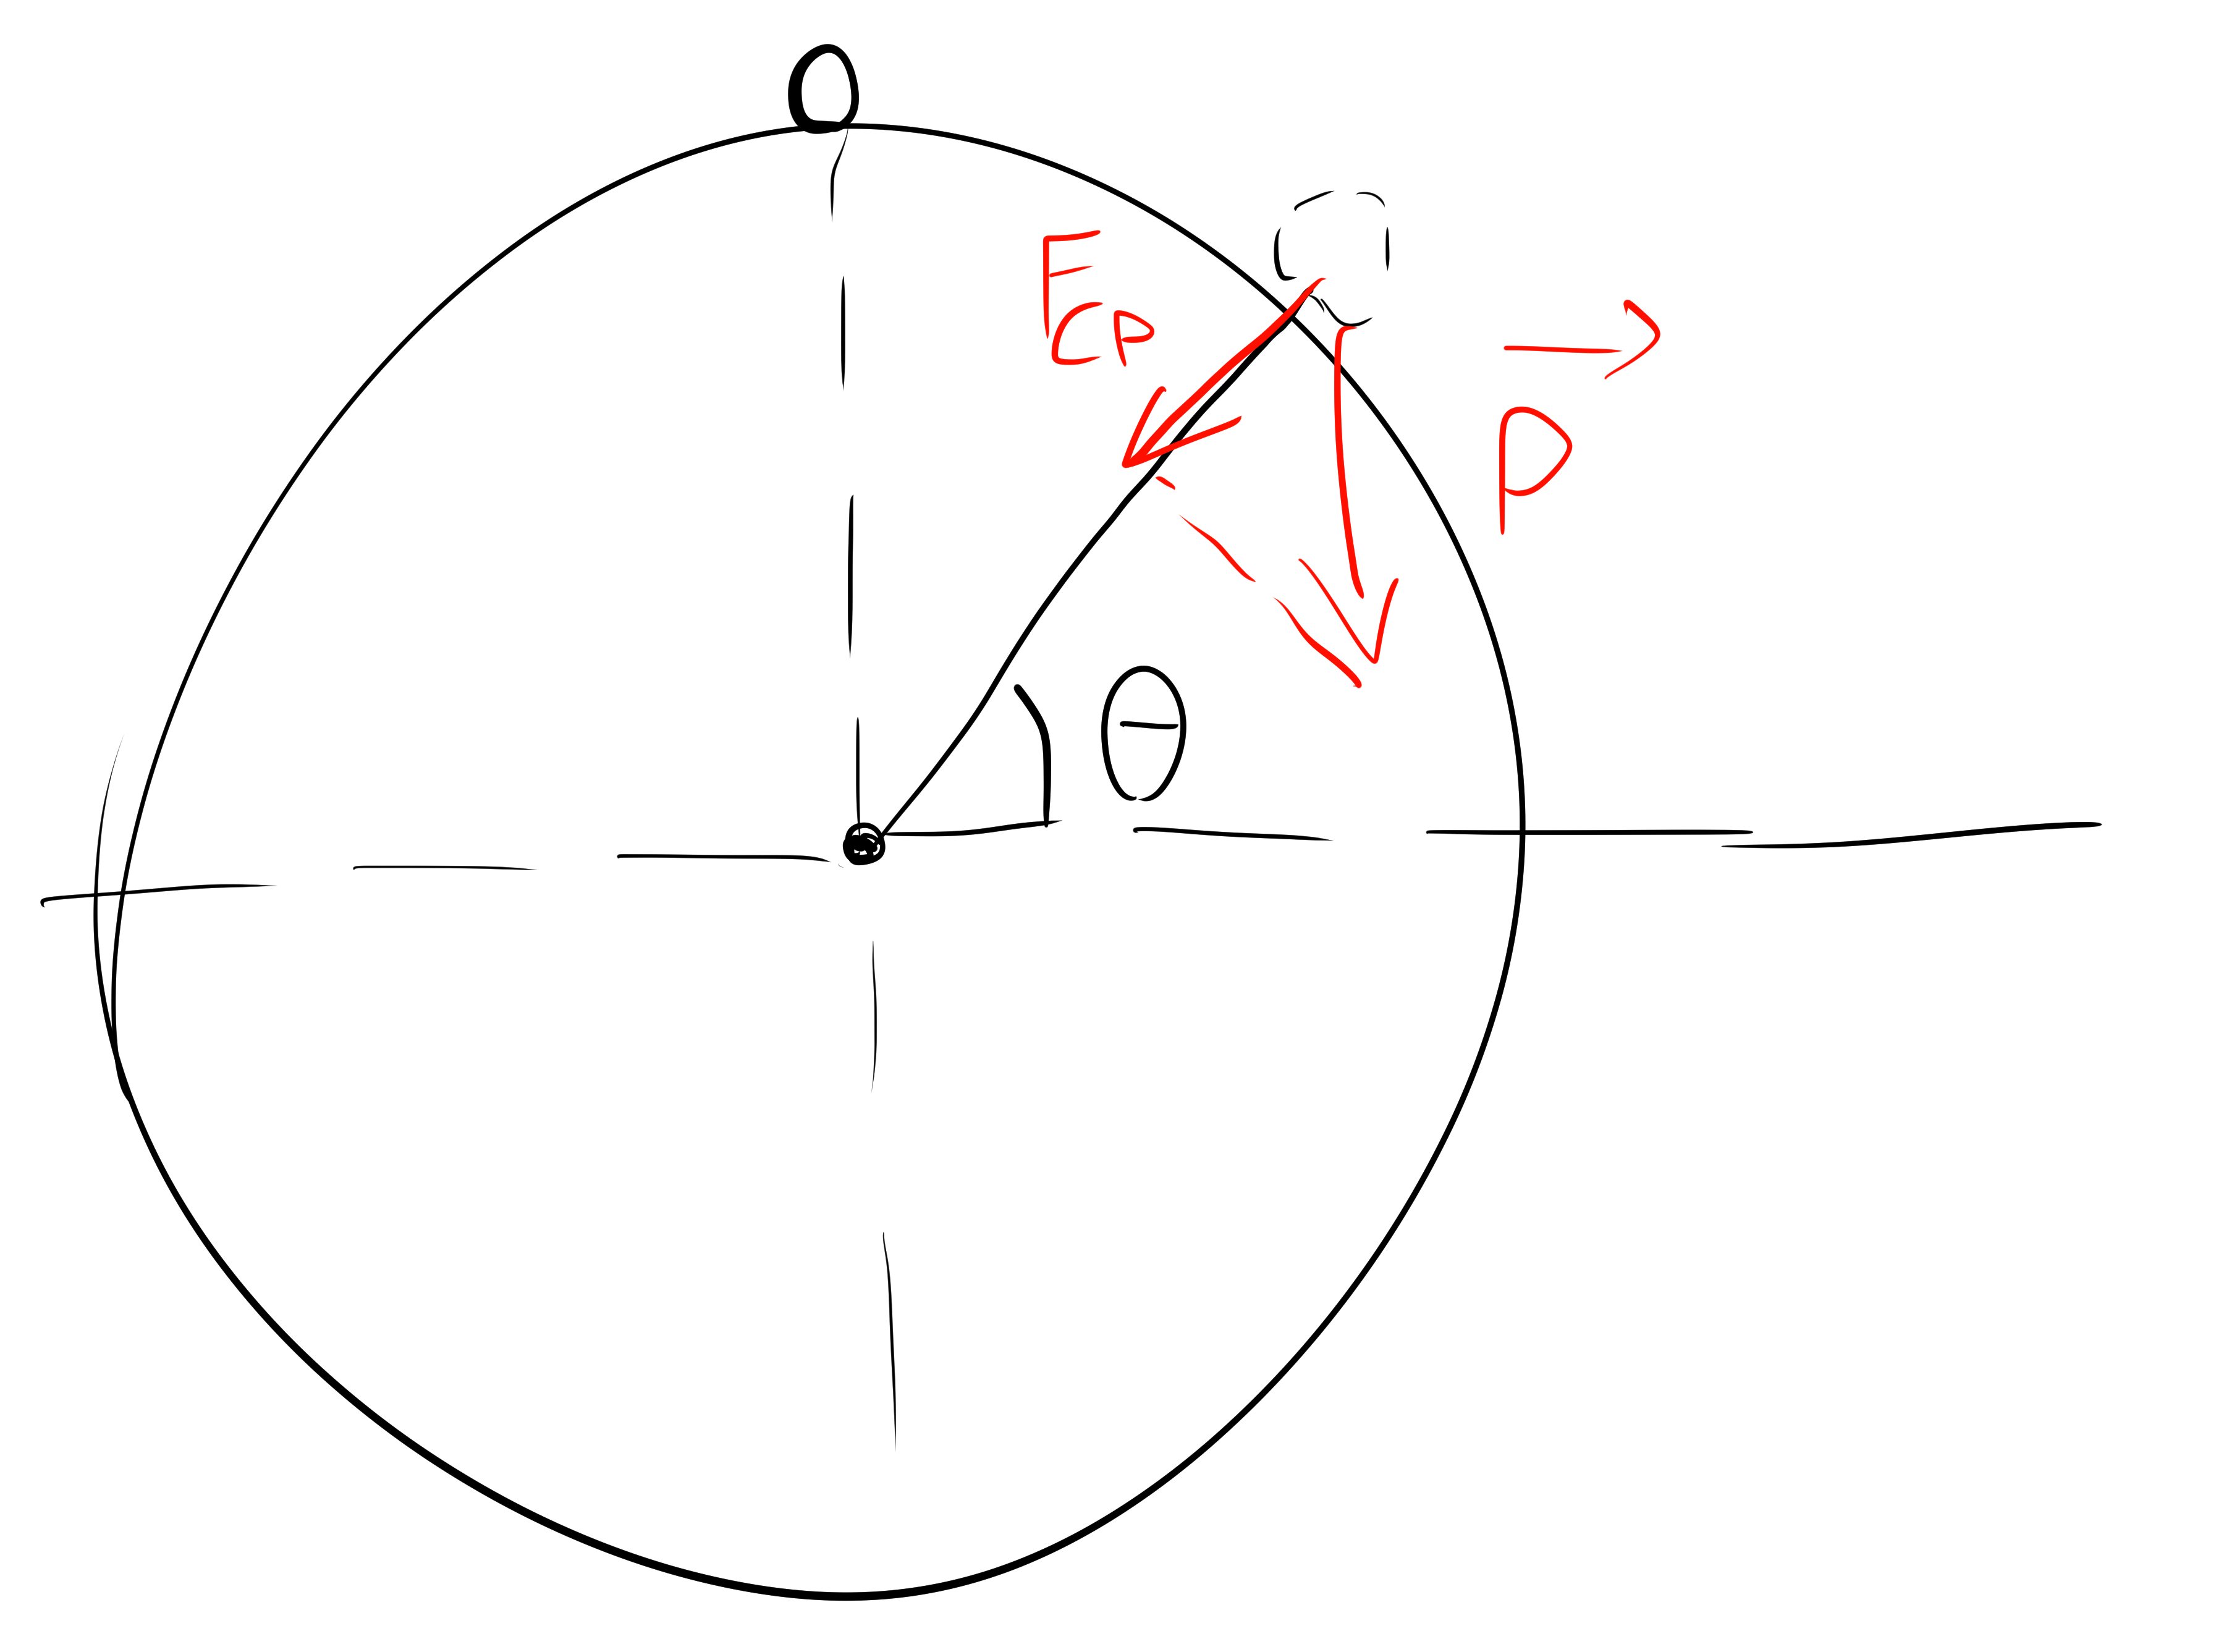
\includegraphics[width=1\linewidth]{fig8}

		\end{multi}

		Sabemos que, enquanto o corpo permanece grudado à superfície da esfera, temos um movimento circular, o que exige uma força centrípeta $ \vec{F_{cp}} $. No caso, tal força centrípeta corresponde à uma das componentes do peso $ \vec{P} $, que aponta para o centro da esfera. Dessa forma
		\begin{align}
			P\sin\theta    & = F_{cp}\implies \nonumber      \\
			m\,g\sin\theta & =m\,\dfrac{v_E^{2}}{R}\nonumber \\
			v_G^{2}        & =R\,g\sin\theta\label{eq:vG2}
		\end{align}
		onde $ v_G $ é a velocidade enquanto o corpo está grudado à esfera.

		Quando o corpo se desgruda da esfera, temos $ v>v_G $, portanto, no momento em que perdem contato,
		\begin{align*}
			v            & =v_G\implies v^{2}=v_D^{2} \\
			\intertext{já que ambas quantidades são positivas. substituindo \ref{eq:v2circle} e \ref{eq:vG2}, temos}
			2g\del{2R-h} & =R\,g\sin\theta            \\
			\intertext{sendo $ h=R+R\sin\theta\implies \sin\theta=\del{h-R}/R $, ficamos com}
			2\del{2R-h}  & =R\del{\dfrac{h-R}{R}}     \\
			h            & =\dfrac{5}{3}R
		\end{align*}
	\end{solution}

	\question Um bloco de massa $ m $ desliza sobre uma mesa horizontal, com coeficientes de atrito cinético, $ \mu_c $, e estático, $ \mu_e $, respectivamente, colide com uma mola de massa desprezível e de constante de mola $ k $, inicialmente na posição relaxada. O bloco atinge a mola com velocidade $ \vec{v_0} $. \begin{enumerate*}[label=(\alph*)]
		\item Qual a deformação máxima da mola? \item Que acontece depois que a mola atinge sua deformação máxima? \item Que fração da energia inicial é dissipada pelo atrito nesse processo? Discuta as situações possíveis.
	\end{enumerate*}

	\begin{solution}
		\changelabel{(\alph*)}
		\un[start=1]
		Supondo que a colisão da massa com o bloco se dá em uma dimensão, vamos definir um sistema de coordenadas com origem na ponta da mola, de tal forma que o movimento anterior do bloco se dava na região negativa do eixo, e após, no sentido positivo%
		\footnote{Note que, como o movimento se dá em uma dimensão, utilizaremos somente o módulo das grandezas discutidas ($ |\vec{v_0}|=v_0 $).}.

		Como não há conservação de energia no sistema, temos que a energia inicial $ E_0 $ será igual à energia final $ E $, acrescida do trabalho realizado pela força dissipativa $ W_{F_{at}\,0\to r} $, no caso, a força de atrito $ F_{at} $, que atua da origem até o ponto de deformação máxima da mola, $ r $. Equacionando, temos
		\begin{equation}\label{eq:enConsFat}
			E_0=E+W_{F_{at}\,0\to r}\implies K_0=K+U_s(r)+\int_{0}^{r}F_{at},
		\end{equation}
		onde $ K,K_0 $ são as energias cinéticas do bloco nos momentos final e inicial, respectivamente, e $ U_s(r) $ é a energia potencial da mola na posição $ r $.

		Dessa forma, temos, por \ref{eq:enConsFat}
		\begin{align*}
			\dfrac{1}{2}m\,v_0^{2}                               & =\dfrac{1}{2}m\,v^{2}+\dfrac{1}{2}k\,r^{2}+\int_{0}^{r}\mu_c\,N\dif r' \\
			\intertext{onde $ v=0 $ é a velocidade final do bloco e $ N $ é a normal do bloco com o plano}
			r^{2}+2\dfrac{\mu_c\,m\,g}{k}r-\dfrac{m}{k}\,v_0^{2} & =0.
		\end{align*}
		De tal forma que
		\begin{align*}
			r & =\dfrac{-2\mu_c\,m\,g/k\pm\sqrt{\del{2\mu_c\,m\,g/k}^{2}+4m\,v_0^{2}/k}}{2}\stackrel{!}{>}0 \\
			r & =\dfrac{-\mu_c\,m\,g+\sqrt{\del{\mu_c\,m\,g}^{2}+m\,k\,v_0^{2}}}{k}
		\end{align*}

		\item Após atingir sua deformação máxima, a mola só voltará a se mover caso sua força seja superior à força máxima de atrito estático $ F_{at\,e} $, proporcionada pela mesa. Sendo a força elástica na ocasião $ F_{el}(r)=-\od{U_s}{x}(r) $, temos a condição:
		\begin{align*}
			F_{at\,e}   & \leqslant F_{el}(r)=-\dod{U_s}{x}(r)                                                                           \\
			\mu_e\,m\,g & \leqslant -\eval{\del{k\,x}}_{x=r}= -k\del{\dfrac{-\mu_c\,m\,g+\sqrt{\del{\mu_c\,m\,g}^{2}+m\,k\,v_0^{2}}}{k}} \\
			\mu_e       & \leqslant \mu_c\del{1-\sqrt{1+k\,v_0^{2}/(\mu_c\,m\,g^{2})}}
		\end{align*}
		E, como $ \mu_c<\mu_e $, e $ 1-\sqrt{1+k\,v_0^{2}/(\mu_c\,m\,g^{2})}<1 $, já que o termo na raiz é positivo, a mola permanece estática, pois a condição nunca será satisfeita na presença de atrito.

		\en
	\end{solution}

	\question Um oscilador harmônico tridimensional isotrópico é definido como uma partícula que se move sob a ação de forças associadas à energia potencial
	\[ U(x, y, z) = \dfrac{1}{2}k(x^2 + y^2 + z^2), \]
	onde $ k $ é uma constante positiva. Mostre que a força correspondente é uma força central e calcule-a. De que tipo é a força obtida?

	\begin{solution}

	\end{solution}



	\question Mostre que o trabalho necessário para remover um objeto da atração gravitacional da Terra é o mesmo que seria necessário para elevá-lo ao topo de uma montanha de altura igual ao raio da Terra, caso a força gravitacional permanecesse constante e igual ao seu valor na superfície da Terra, durante a escalada da montanha.

	\begin{solution}

	\end{solution}

\end{questions}
\end{document}
